\documentclass[compress]{beamer}
\usepackage{ifthen,verbatim}

\newcommand{\isnote}{}
\xdefinecolor{lightyellow}{rgb}{1.,1.,0.25}
\xdefinecolor{darkblue}{rgb}{0.1,0.1,0.7}

%% Uncomment this to get annotations
%% \def\notes{\addtocounter{page}{-1}
%%            \renewcommand{\isnote}{*}
%% 	   \beamertemplateshadingbackground{lightyellow}{white}
%%            \begin{frame}
%%            \frametitle{Notes for the previous page (page \insertpagenumber)}
%%            \itemize}
%% \def\endnotes{\enditemize
%% 	      \end{frame}
%%               \beamertemplateshadingbackground{white}{white}
%%               \renewcommand{\isnote}{}}

%% Uncomment this to not get annotations
\def\notes{\comment}
\def\endnotes{\endcomment}

\setbeamertemplate{navigation symbols}{}
\setbeamertemplate{headline}{\mbox{ } \hfill
\begin{minipage}{5.5 cm}
\vspace{-0.75 cm} \small
\end{minipage} \hfill
\begin{minipage}{4.5 cm}
\vspace{-0.75 cm} \small
\begin{flushright}
\ifthenelse{\equal{\insertpagenumber}{1}}{}{Jim Pivarski \hspace{0.2 cm} \insertpagenumber\isnote/\pageref{numpages}}
\end{flushright}
\end{minipage}\mbox{\hspace{0.2 cm}}\includegraphics[height=1 cm]{../cmslogo} \hspace{0.1 cm} \includegraphics[height=1 cm]{../tamulogo} \hspace{0.01 cm} \vspace{-1.05 cm}}

\begin{document}
\begin{frame}
\vfill
\begin{center}
\textcolor{darkblue}{\Large Track-based Alignment Paper}

\vfill
\begin{columns}
\column{0.3\linewidth}
\begin{center}
\large
\textcolor{darkblue}{Jim Pivarski}
\end{center}
\column{0.3\linewidth}
\begin{center}
\large
Gervasio Gomez
\end{center}
\end{columns}

\begin{columns}
\column{0.3\linewidth}
\begin{center}
\scriptsize
{\it Texas A\&M University}
\end{center}
\column{0.3\linewidth}
\begin{center}
\scriptsize
{\it Instituto de Fisica de Cantabria}
\end{center}
\end{columns}

\vfill
23 July, 2009

\end{center}
\end{frame}

%% \begin{notes}
%% \item This is the annotated version of my talk.
%% \item If you want the version that I am presenting, download the one
%% labeled ``slides'' on Indico (or just ignore these yellow pages).
%% \item The annotated version is provided for extra detail and a written
%% record of comments that I intend to make orally.
%% \item Yellow notes refer to the content on the {\it previous} page.
%% \item All other slides are identical for the two versions.
%% \end{notes}

\small

\begin{frame}
\frametitle{Contents and structure}

\vspace{0.25 cm}
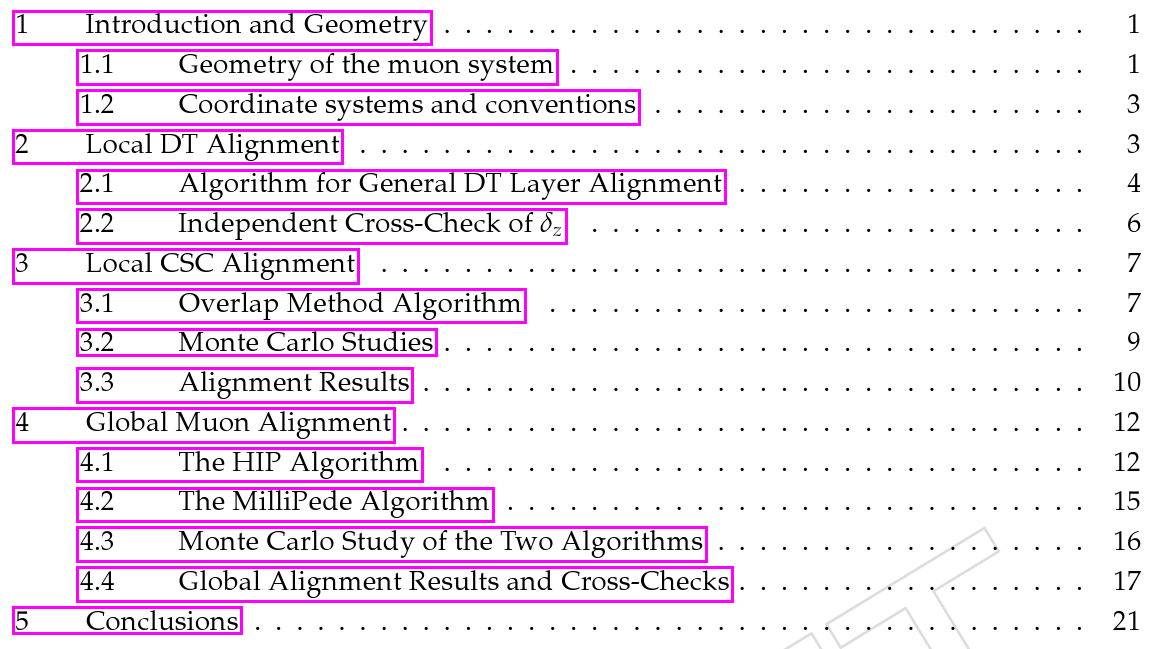
\includegraphics[width=0.9\linewidth]{contents.png}

\begin{itemize}
\item Two independent sections on local alignments
\item One section on global alignment with both procedures
\begin{itemize}
\item algorithms are described separately
\item MC studies and results are shown together
\end{itemize}
\item 24 pages, 12 figures
\end{itemize}

%% \hspace{-0.83 cm} \textcolor{darkblue}{\Large Outline2}
\end{frame}

\begin{frame}
\frametitle{Local DT alignment}
\framesubtitle{Alignment of layers and superlayers in chambers}

\begin{itemize}
\item Two alignments described:
\begin{enumerate}
\item layer alignment, including information from tracks, quality control measurements, and photogrammetry
\item superlayer alignment, using tracks and photogrammetry independently, then cross-checked
\end{enumerate}

\item Tracks alone are not sufficient to align layers and fit tracks simultaneously: consider shear distortion
\begin{center}
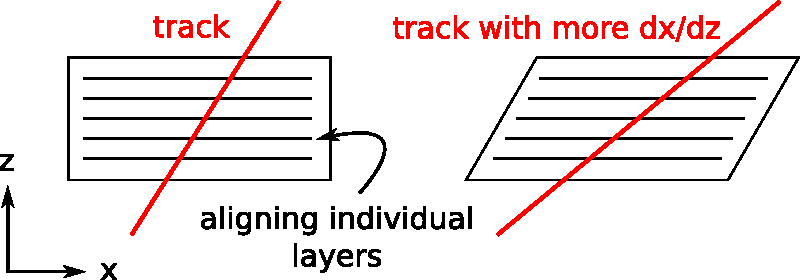
\includegraphics[width=0.6\linewidth]{shear.pdf}
\end{center}

\item Because \textcolor{darkblue}{(1)} uses all of the available data sources, no cross-checks are possible

\item Alignment \textcolor{darkblue}{(2)} uses 2-D segment from each
  superlayer to determine $x$, $\phi_z$, and especially $z$ (width of
  glue layer)

\end{itemize}
\end{frame}

\begin{frame}
\frametitle{Local DT alignment}

\vfill
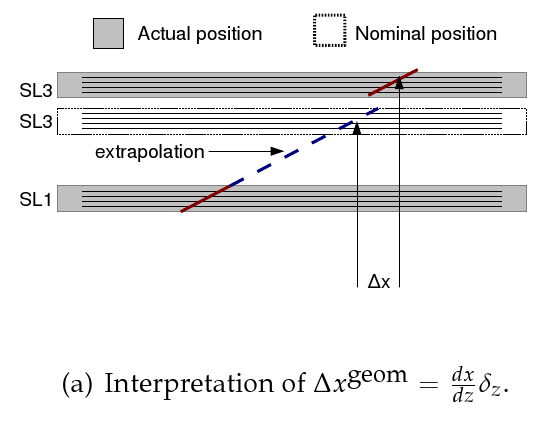
\includegraphics[width=0.45\linewidth]{dtsuperlayer.png}
\hfill 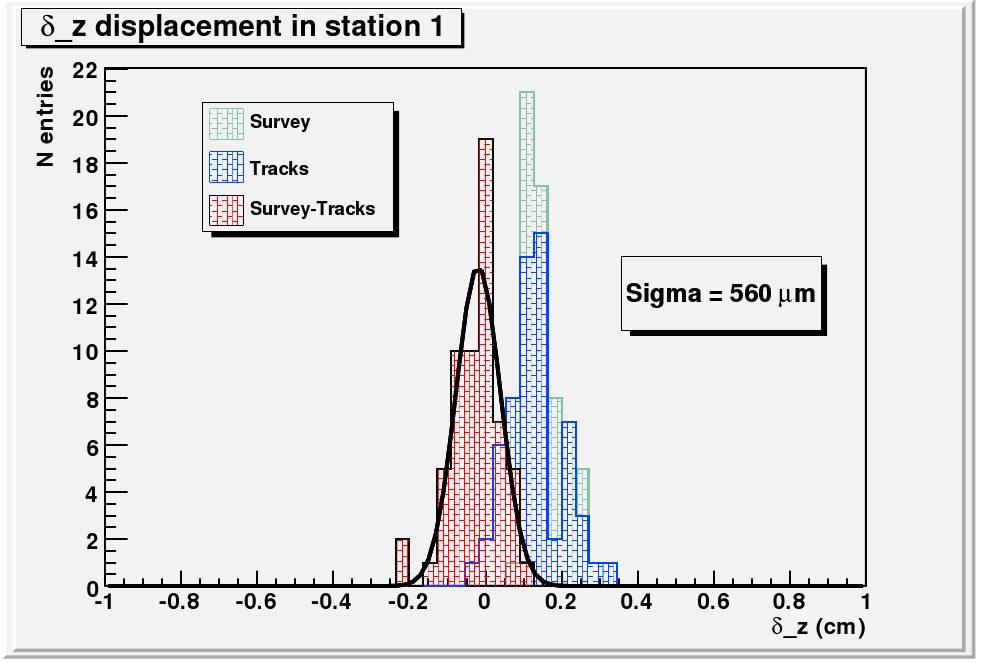
\includegraphics[width=0.5\linewidth]{dtinternal_crosscheck.png}

\vfill
\begin{itemize}
\item Superlayer alignment can be performed purely with tracks because each superlayer defines a line with slope ($\frac{dx}{dz}$)
\begin{itemize}
\item discrepancies between segments $\to$ $x$ corrections
\item \ldots as a function of $y$ $\to$ $\phi_z$ corrections
\item \ldots as a function of $\frac{dx}{dz}$ $\to$ $z$ corrections
\end{itemize}
\item Good agreement with photogrammetry for all 3 parameters
\item Only $z$ was significant (due to glue layer)
\end{itemize}
\end{frame}

\begin{frame}
\frametitle{Local CSC alignment}
\framesubtitle{Alignment of chambers in rings}

\hfill 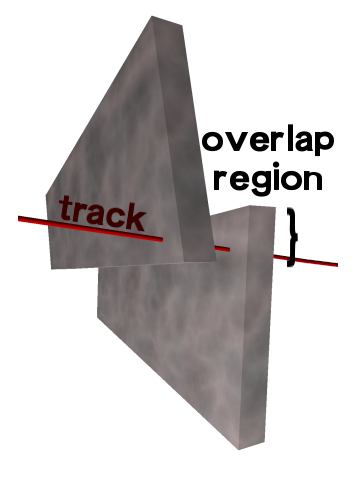
\includegraphics[height=2.5 cm]{overlaps.png}

\vspace{-2.5 cm}
\begin{itemize}
\item Uses overlap of neighboring chambers for precise \\ relative alignments
\item Relative corrections propagated around the ring \\ (full mathematical detail given in note)
\item Tracks-only measurement compares favorably with \\ photogrammetry ($\vec{B}=0$ beam-halo)

\mbox{\hspace{-0.75 cm}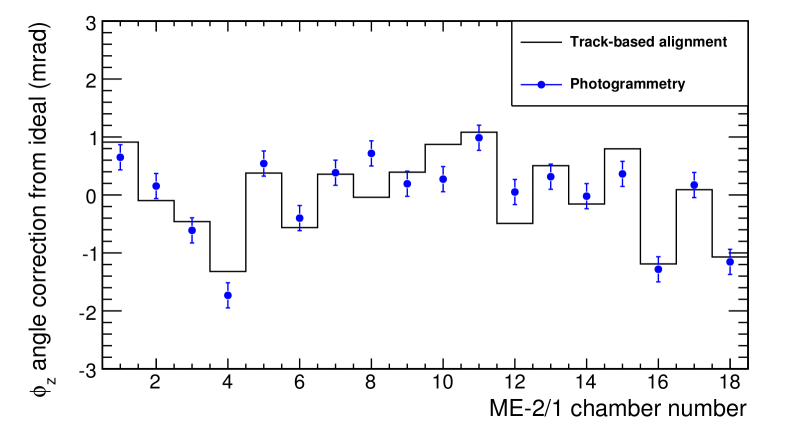
\includegraphics[height=3 cm]{data_correlations.png}
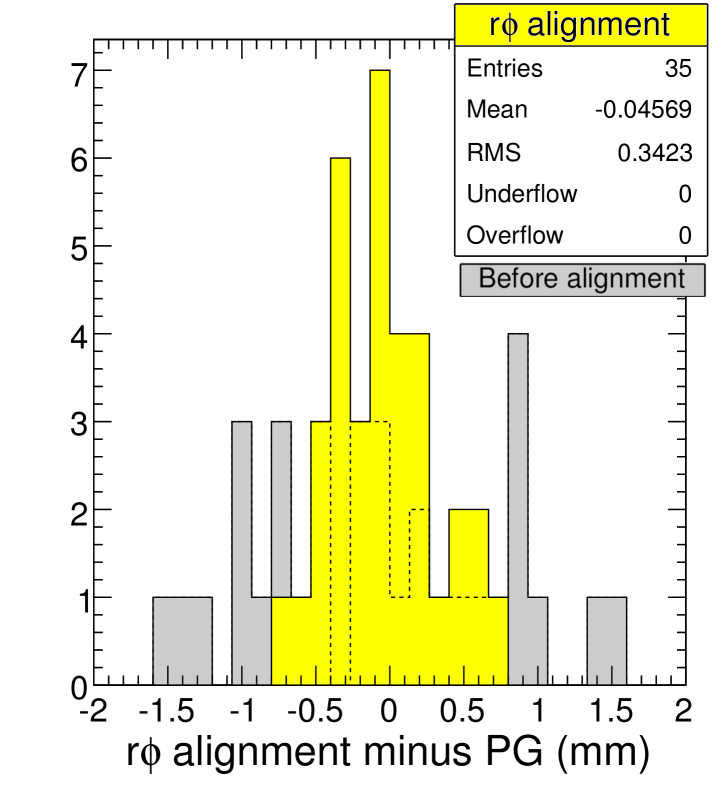
\includegraphics[height=3 cm]{data_rphi.png}
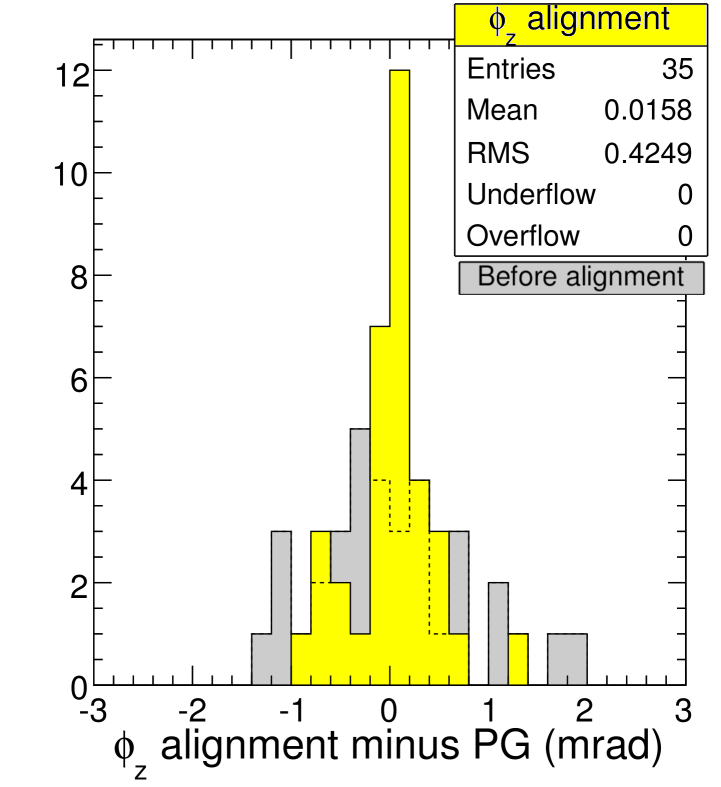
\includegraphics[height=3 cm]{data_phiz.png}}

\item Includes a Monte Carlo study
\item Extension to layer alignment mentioned, but not developed (would require more beam-halo to demonstrate)
\end{itemize}
\end{frame}

\begin{frame}
\frametitle{Global alignment: algorithms}

\begin{columns}
\column{0.55\linewidth}
\begin{itemize}
\item 2 sections: HIP and MillePede
\item \mbox{Complete description of Muon-HIP,\hspace{-1 cm}} \\ how it differs from standard HIP:
\begin{itemize}\setlength{\itemsep}{0.1 cm}
\item tracks fixed by tracker
\item treatment of segment residuals: \mbox{$\Delta x$, $\Delta y$, $\Delta \frac{dx}{dz}$, $\Delta \frac{dy}{dz}$\hspace{-1 cm}}

including CSC case

\item fit function: convolution of misalignment and propagation errors
\item sample fits (data only)
\end{itemize}

\item Complete description of MillePede:

\vspace{-0.2 cm}
\begin{itemize}
\item how it differs from the general case (fixed tracks)
\item list of potential systematic errors
\end{itemize}
\end{itemize}

\column{0.5\linewidth}
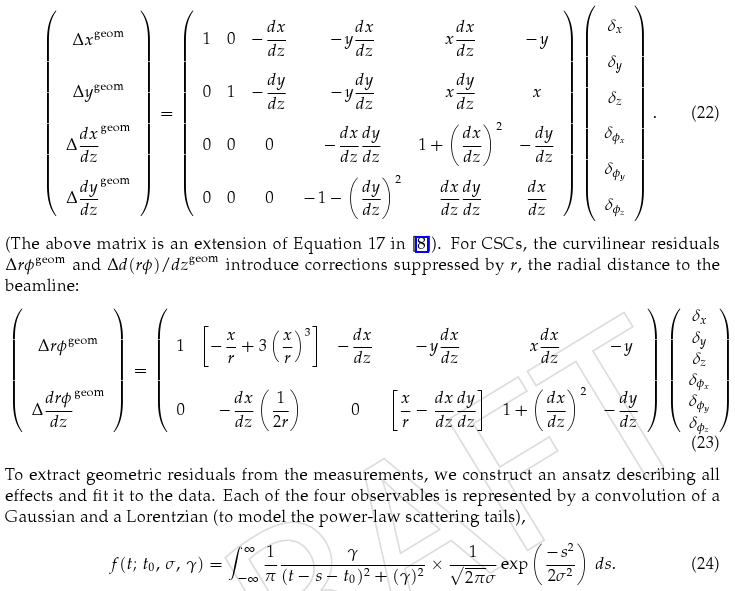
\includegraphics[width=\linewidth]{hipalgo.png}

\vspace{0.5 cm}
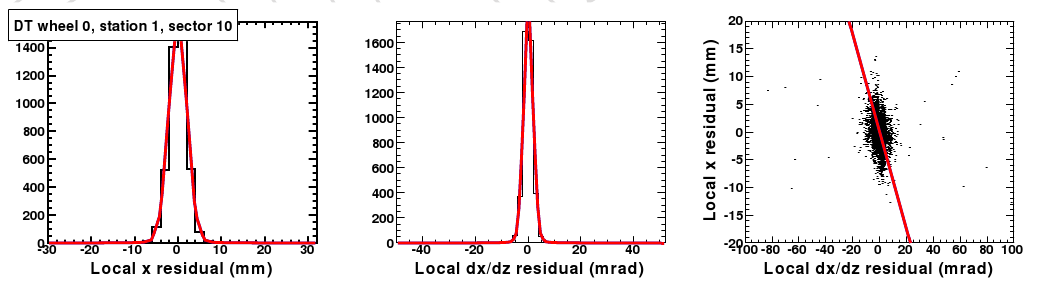
\includegraphics[width=\linewidth]{samplefits.png}

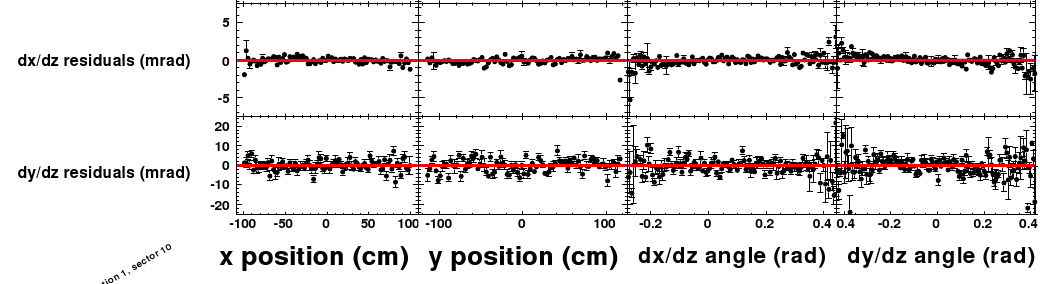
\includegraphics[width=\linewidth]{samplefits2.png}
\end{columns}
\end{frame}

\begin{frame}
\frametitle{Parallel MC studies}

\begin{columns}
\column{0.6\linewidth}

\textcolor{darkblue}{HIP:}

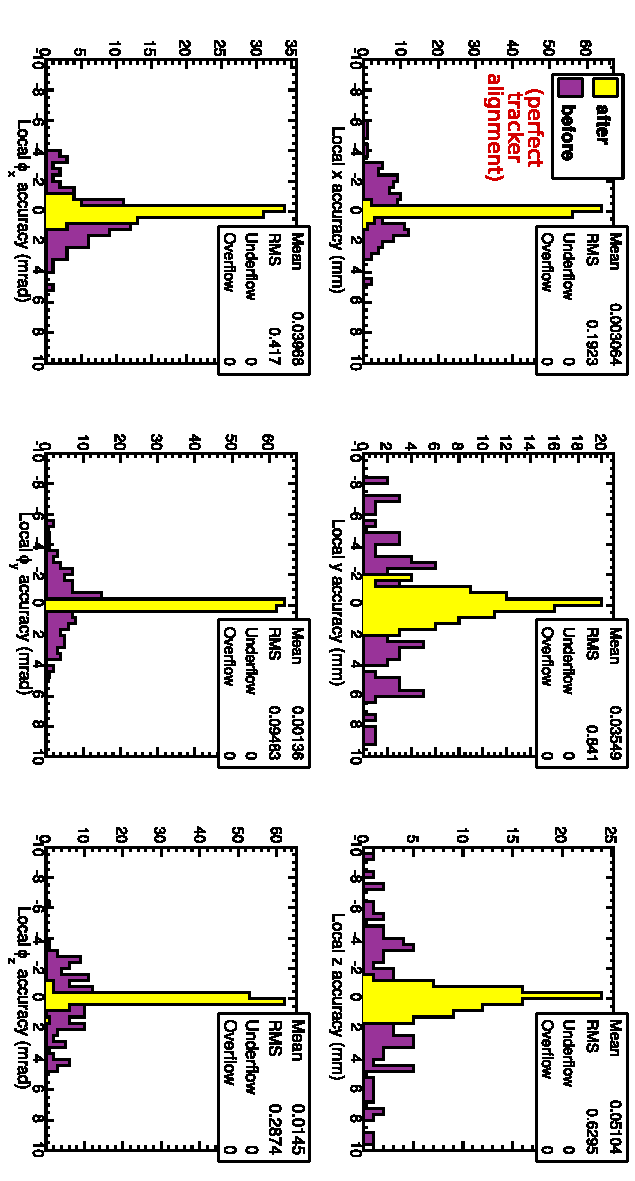
\includegraphics[height=\linewidth, angle=90]{hip_MC.pdf}

\vfill
\textcolor{darkblue}{Millepede:}

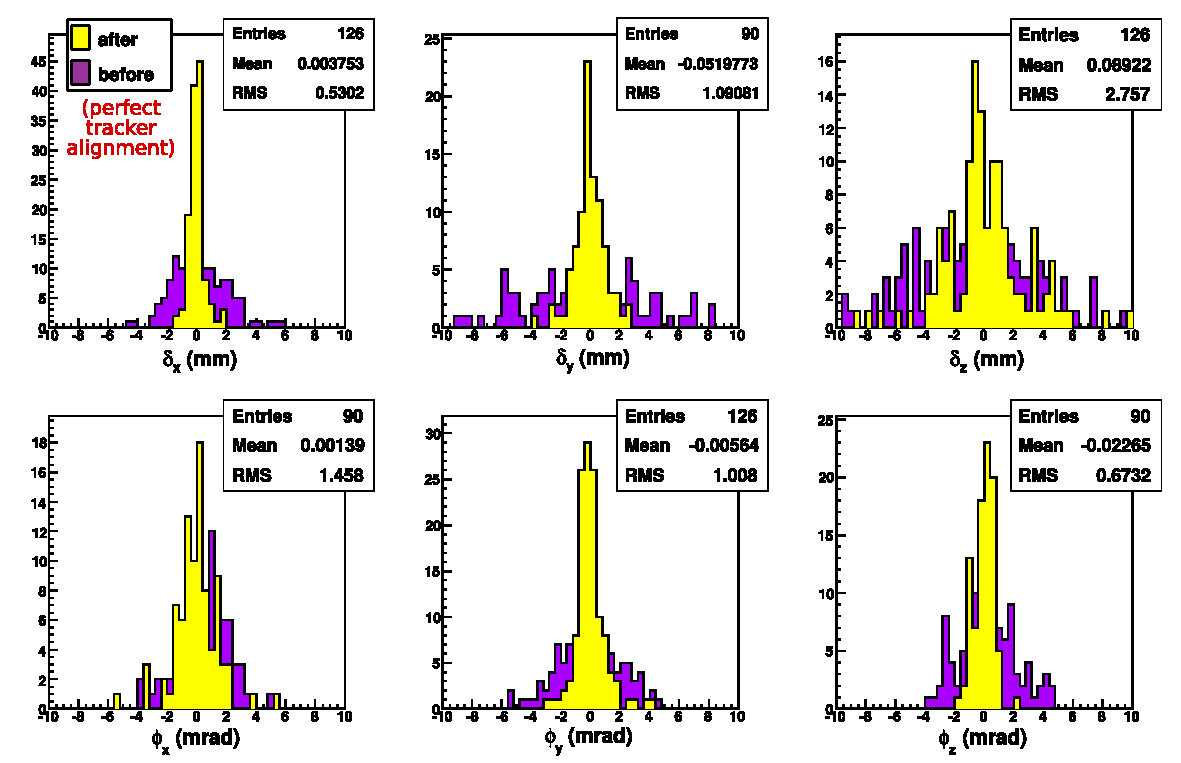
\includegraphics[width=\linewidth]{Millipede_MC_RandomScenario.pdf}

\column{0.43\linewidth}

\begin{itemize}
\item Cosmic ray Monte Carlo
\item Everything the same as data except no tracker misalignment, \mbox{$\vec{B}(\vec{x})$ errors,\hspace{-1 cm}} \\ or \mbox{internal DT misalignment\hspace{-2 cm}}
\item Width of difference between aligned and true:
\end{itemize}

\begin{tabular}{c c c c}
& HIP & MP & \\\hline
$\delta_x$ & 0.19 & 0.53 & mm \\
$\delta_y$ & 0.84 & 1.09 & mm \\
$\delta_z$ & 0.63 & 2.76 & mm \\
$\delta_{\phi_x}$ & 0.42 & 1.46 & mrad \\
$\delta_{\phi_y}$ & 0.09 & 1.01 & mrad \\
$\delta_{\phi_z}$ & 0.29 & 0.67 & mrad \\
\end{tabular}

\end{columns}
\end{frame}

\begin{frame}
\frametitle{Results (cross-checks)}
\begin{itemize}
\item Since the output of alignment is a many-parameter geometry which
  doesn't mean much to an outside reader, what we show in the Results
  section are cross-checks
\item First check (internal consistency): residuals minimized
\item Second: algorithms agree (within uncertainties set by MC)
\end{itemize}

\mbox{ } \hfill 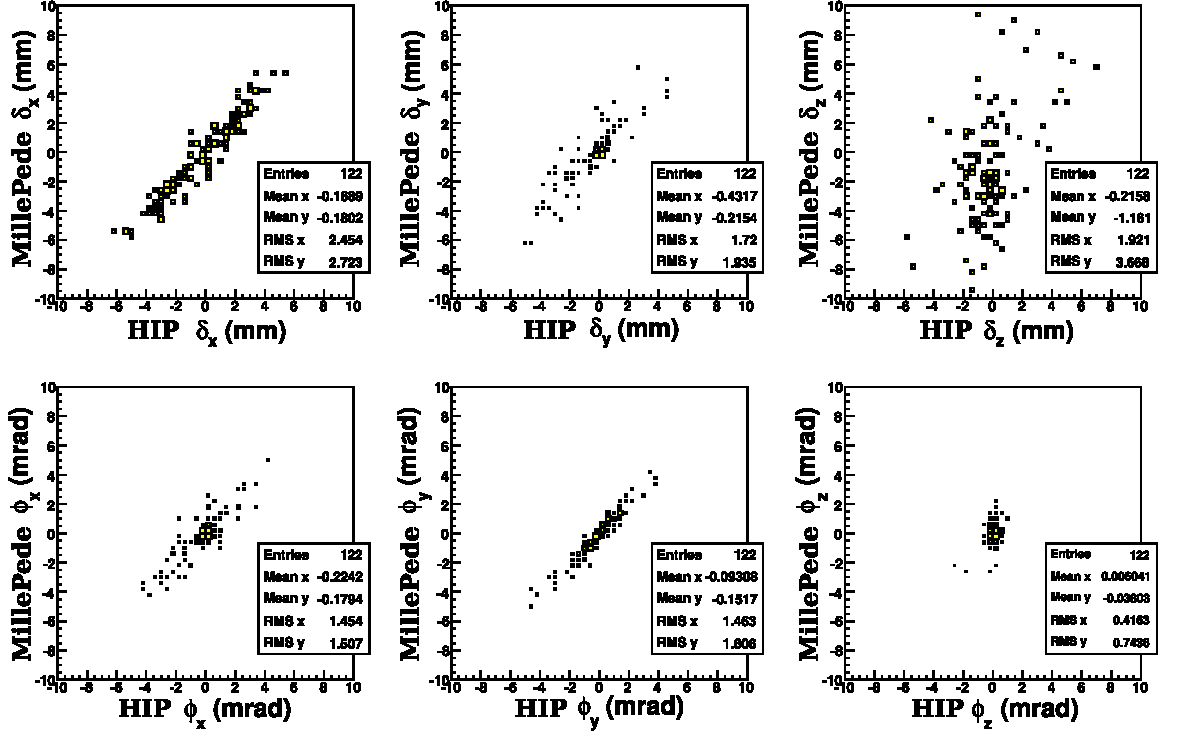
\includegraphics[width=0.8\linewidth]{MP-V4_vs_HIP-V4.pdf} \hfill \mbox{ }
\end{frame}

\begin{frame}
\frametitle{Results (cross-checks)}

\begin{columns}
\column{0.4\linewidth}
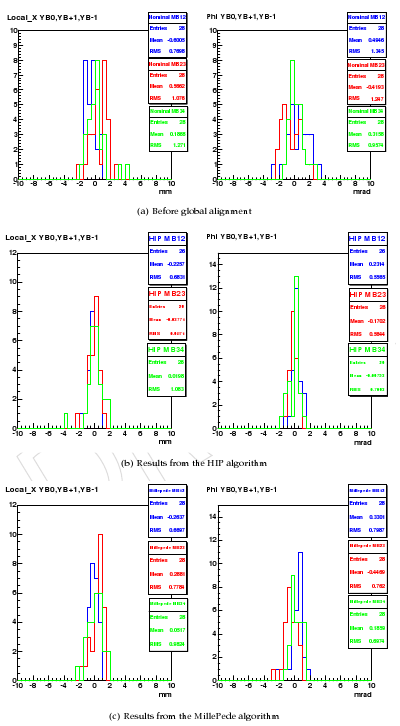
\includegraphics[width=\linewidth]{localcheck.png}

\column{0.6\linewidth}
\begin{itemize}
\item Third check: local and global agree
\begin{itemize}
\item local track fits are partly independent of global track fits
\item higher precision from shorter propagation through only one layer of iron
\item can only quantify relative positions
\end{itemize}

\item Local differences maintained (and slightly improved) despite
  few-mm scale global corrections
\end{itemize}

\begin{center}
\tiny
\begin{tabular}{c c c}
& $x$ (mm) & $\phi_y$ (mrad) \\\hline
before align $1-2$ & 0.77 & 1.35 \\
before align $2-3$ & 1.08 & 1.25 \\
before align $3-4$ & 1.27 & 0.96 \\\hline
HIP $1-2$ & 0.68 & 0.56 \\
HIP $2-3$ & 0.69 & 0.56 \\
HIP $3-4$ & 1.09 & 0.71 \\\hline
Millepede $1-2$ & 0.67 & 0.80 \\
Millepede $2-3$ & 0.78 & 0.76 \\
Millepede $3-4$ & 0.98 & 0.70
\end{tabular}
\end{center}
\end{columns}
\end{frame}

\begin{frame}
\frametitle{Results (cross-checks)}

\begin{itemize}
\item Fourth: split each cosmic ray into two LHC-like halves, fit top and bottom independently
\begin{itemize}
\item any mismatch in $1/p_T$ is purely instrumental
\item select $p_T \gtrsim 200$~GeV to emphasize contribution of the muon alignment (long lever arm for resolution of small sagitta
\end{itemize}
\end{itemize}

\vspace{-0.5 cm}
\begin{columns}
\column{0.4\linewidth}
\begin{center}
\textcolor{darkblue}{Before muon alignment}

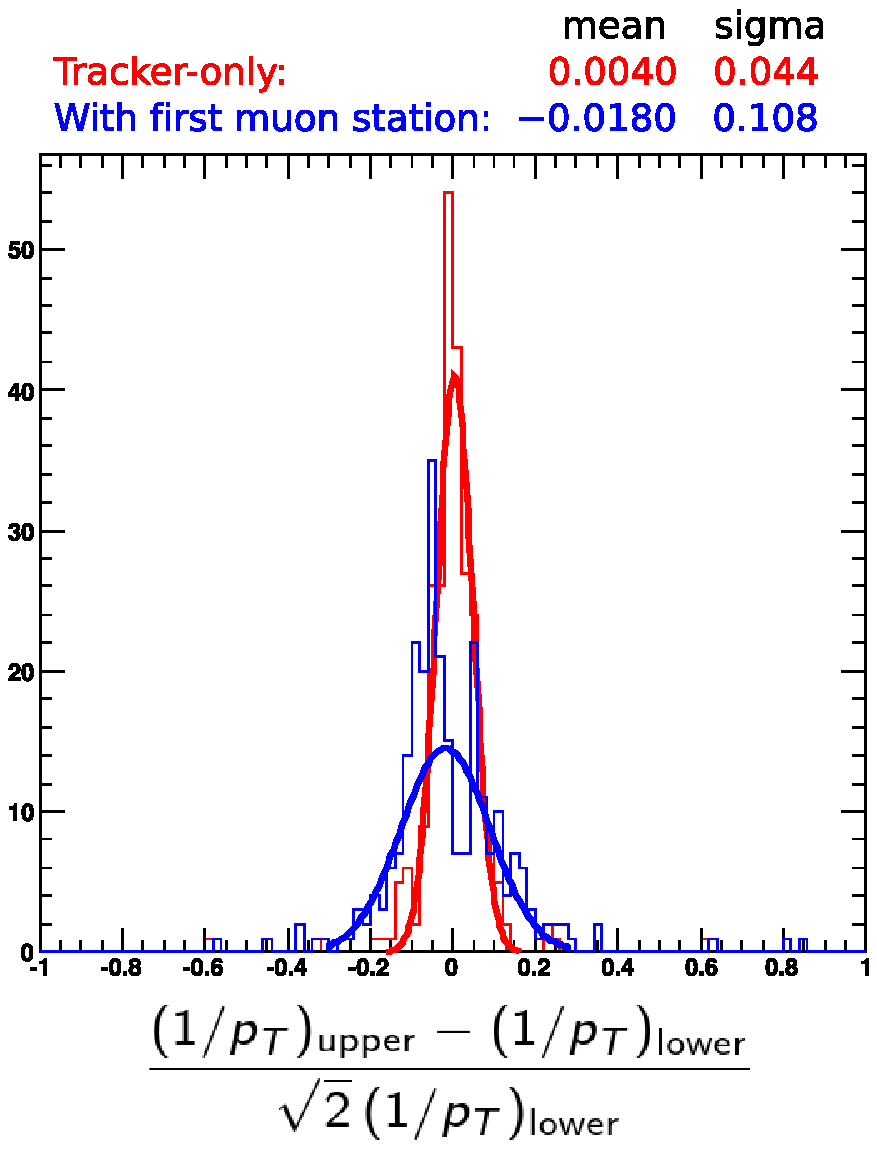
\includegraphics[width=\linewidth]{without_alignment.pdf}
\end{center}
\column{0.4\linewidth}
\begin{center}
\textcolor{darkblue}{After muon alignment}

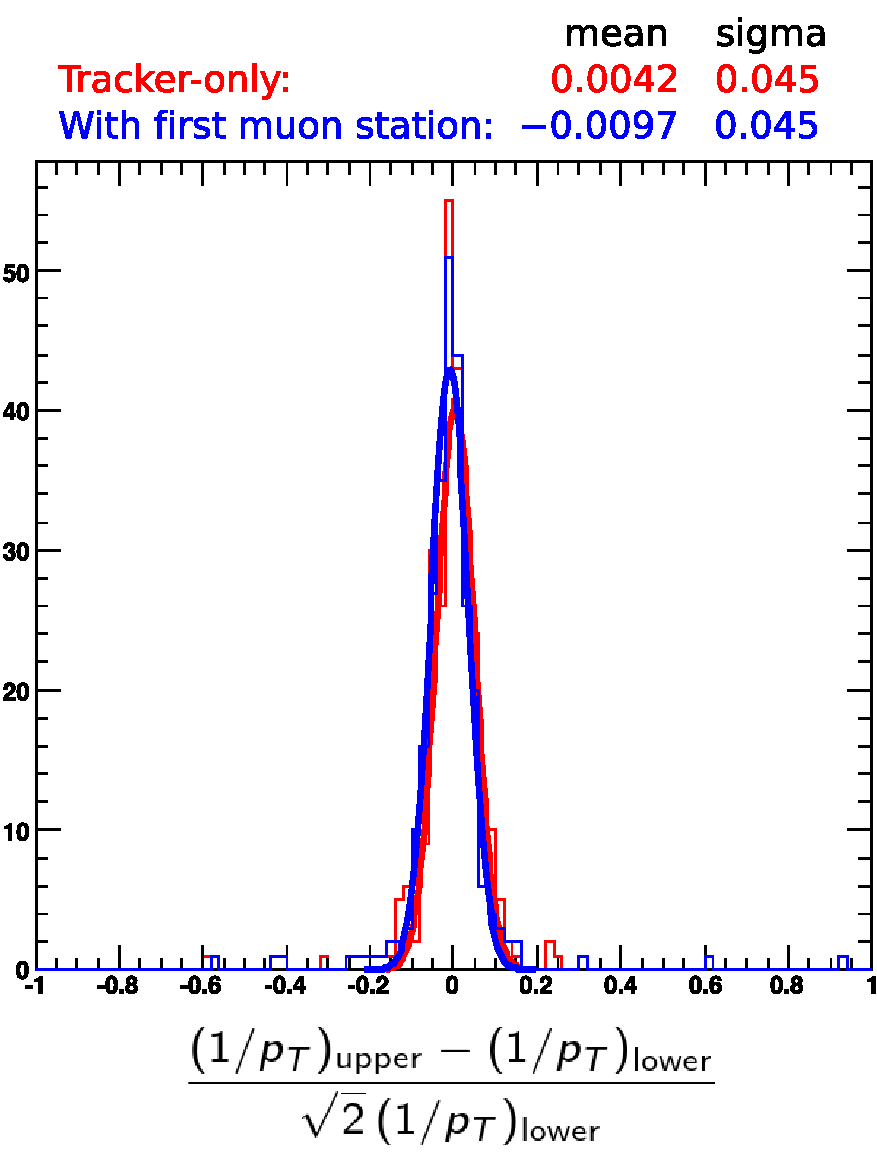
\includegraphics[width=\linewidth]{with_alignment.pdf}
\end{center}

\column{0.3\linewidth}
\mbox{ }

\vspace{0.15 cm}
\scriptsize \centering \textcolor{darkblue}{Plot from Technical Design Report}

\textcolor{darkblue}{(no misalignment)}

\vspace{0.2 cm}
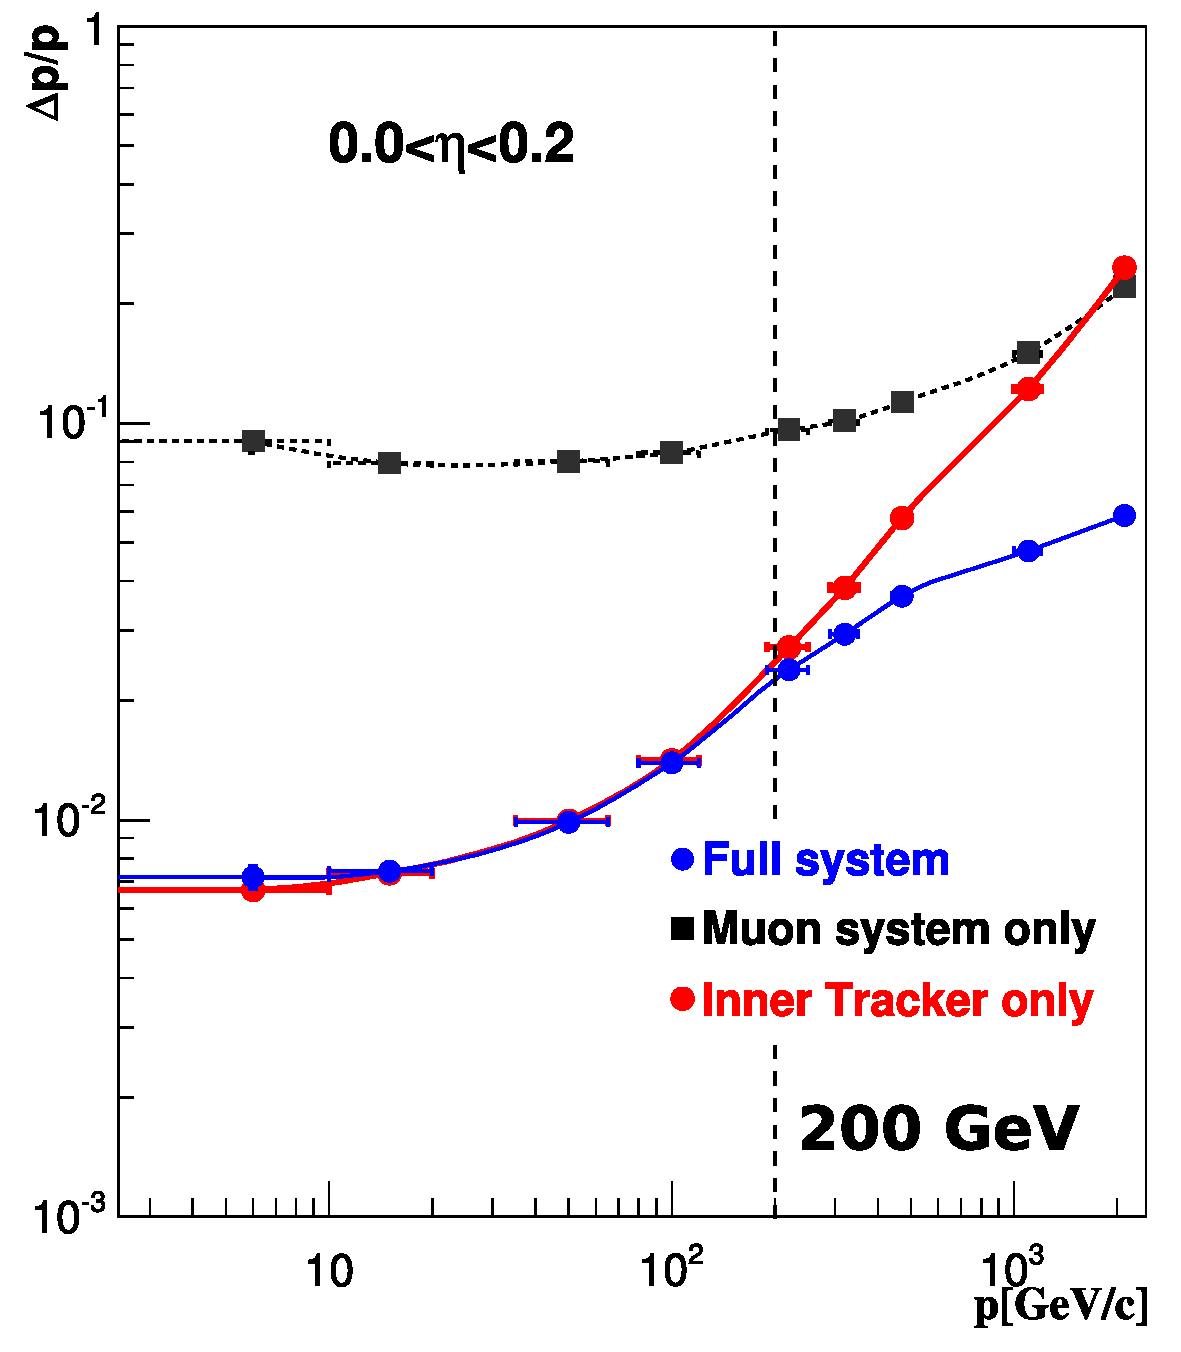
\includegraphics[width=\linewidth]{Figure_001-005-a.pdf}

sigma $\sim$ 0.025 at 200~GeV for a perfect detector
\end{columns}
\end{frame}

%% \section*{First section}
%% \begin{frame}
%% \begin{center}
%% \Huge \textcolor{blue}{First section}
%% \end{center}
%% \end{frame}

\begin{frame}
\frametitle{Conclusions}

\begin{itemize}\setlength{\itemsep}{0.25 cm}
\item This paper contains many mature analyses, demonstrating the quality of our detectors and tracking, and should be published
\item Later than nominal CRAFT paper schedule (our apologies!):
\end{itemize}

\vfill \renewcommand{\arraystretch}{1.25}
\begin{tabular}{p{0.7\linewidth} c}
DPG/POG reading/review/Pre-approval & July 1 \\
ARC Review & July 15--Aug 15 \\
Collaboration-wide review & Aug 20--Sep 6 \\
Final Tar Ball of Paper to Editors & Sep 20 \\
48 Hour notice for final urgent comments & Sep 24 \\
Submission to J.INST & Sept 30
\end{tabular}

\label{numpages}
\end{frame}

\end{document}
